% Gemini theme
% https://github.com/anishathalye/gemini
%
% We try to keep this Overleaf template in sync with the canonical source on
% GitHub, but it's recommended that you obtain the template directly from
% GitHub to ensure that you are using the latest version.

\documentclass[final, 20pt]{beamer}

% ====================
% Packages
% ====================

\usepackage[T1]{fontenc}
\usepackage{lmodern}
% \usepackage[size=custom,width=120,height=72,scale=1.0]{beamerposter}
\usepackage[size=a1,scale=1.3]{beamerposter}
\usetheme{gemini}
\usecolortheme{gemini}
\usepackage{graphicx}
\graphicspath{images}
\usepackage{booktabs}
\usepackage{tikz}
\usepackage{pgfplots}
\usepackage{lipsum}
\usepackage{subcaption}
% ====================
% Lengths
% ====================

% If you have N columns, choose \sepwidth and \colwidth such that
% (N+1)*\sepwidth + N*\colwidth = \paperwidth
\newlength{\sepwidth}
\newlength{\colwidth}
\setlength{\sepwidth}{0.025\paperwidth}
\setlength{\colwidth}{0.3\paperwidth}

\newcommand{\separatorcolumn}{\begin{column}{\sepwidth}\end{column}}

% ====================
% Title
% ====================

\title{Autonomous Drone Landing}

\author{Joshua Springer}

\institute[shortinst]{Reykjavík University}

% ====================
% Body
% ====================

\begin{document}

\begin{frame}[t]
\begin{columns}[t]
\separatorcolumn

\begin{column}{\colwidth}

  \begin{alertblock}{Drone Platforms}
    We have built two Tarot 680 Hexacopters for real world testing of autonomous navigation techniques developed in simulation.
    A landing pad is marked with fiducial markers which are recognized by the drone's onboard camera.
    The gimbal automatically aims the camera at the landing pad to track it during descent.
    The landing software then directs the drone to descend towards the landing pad.

    \begin{figure}
      \includegraphics[width=0.45\linewidth]{images/jetson_electronics}
      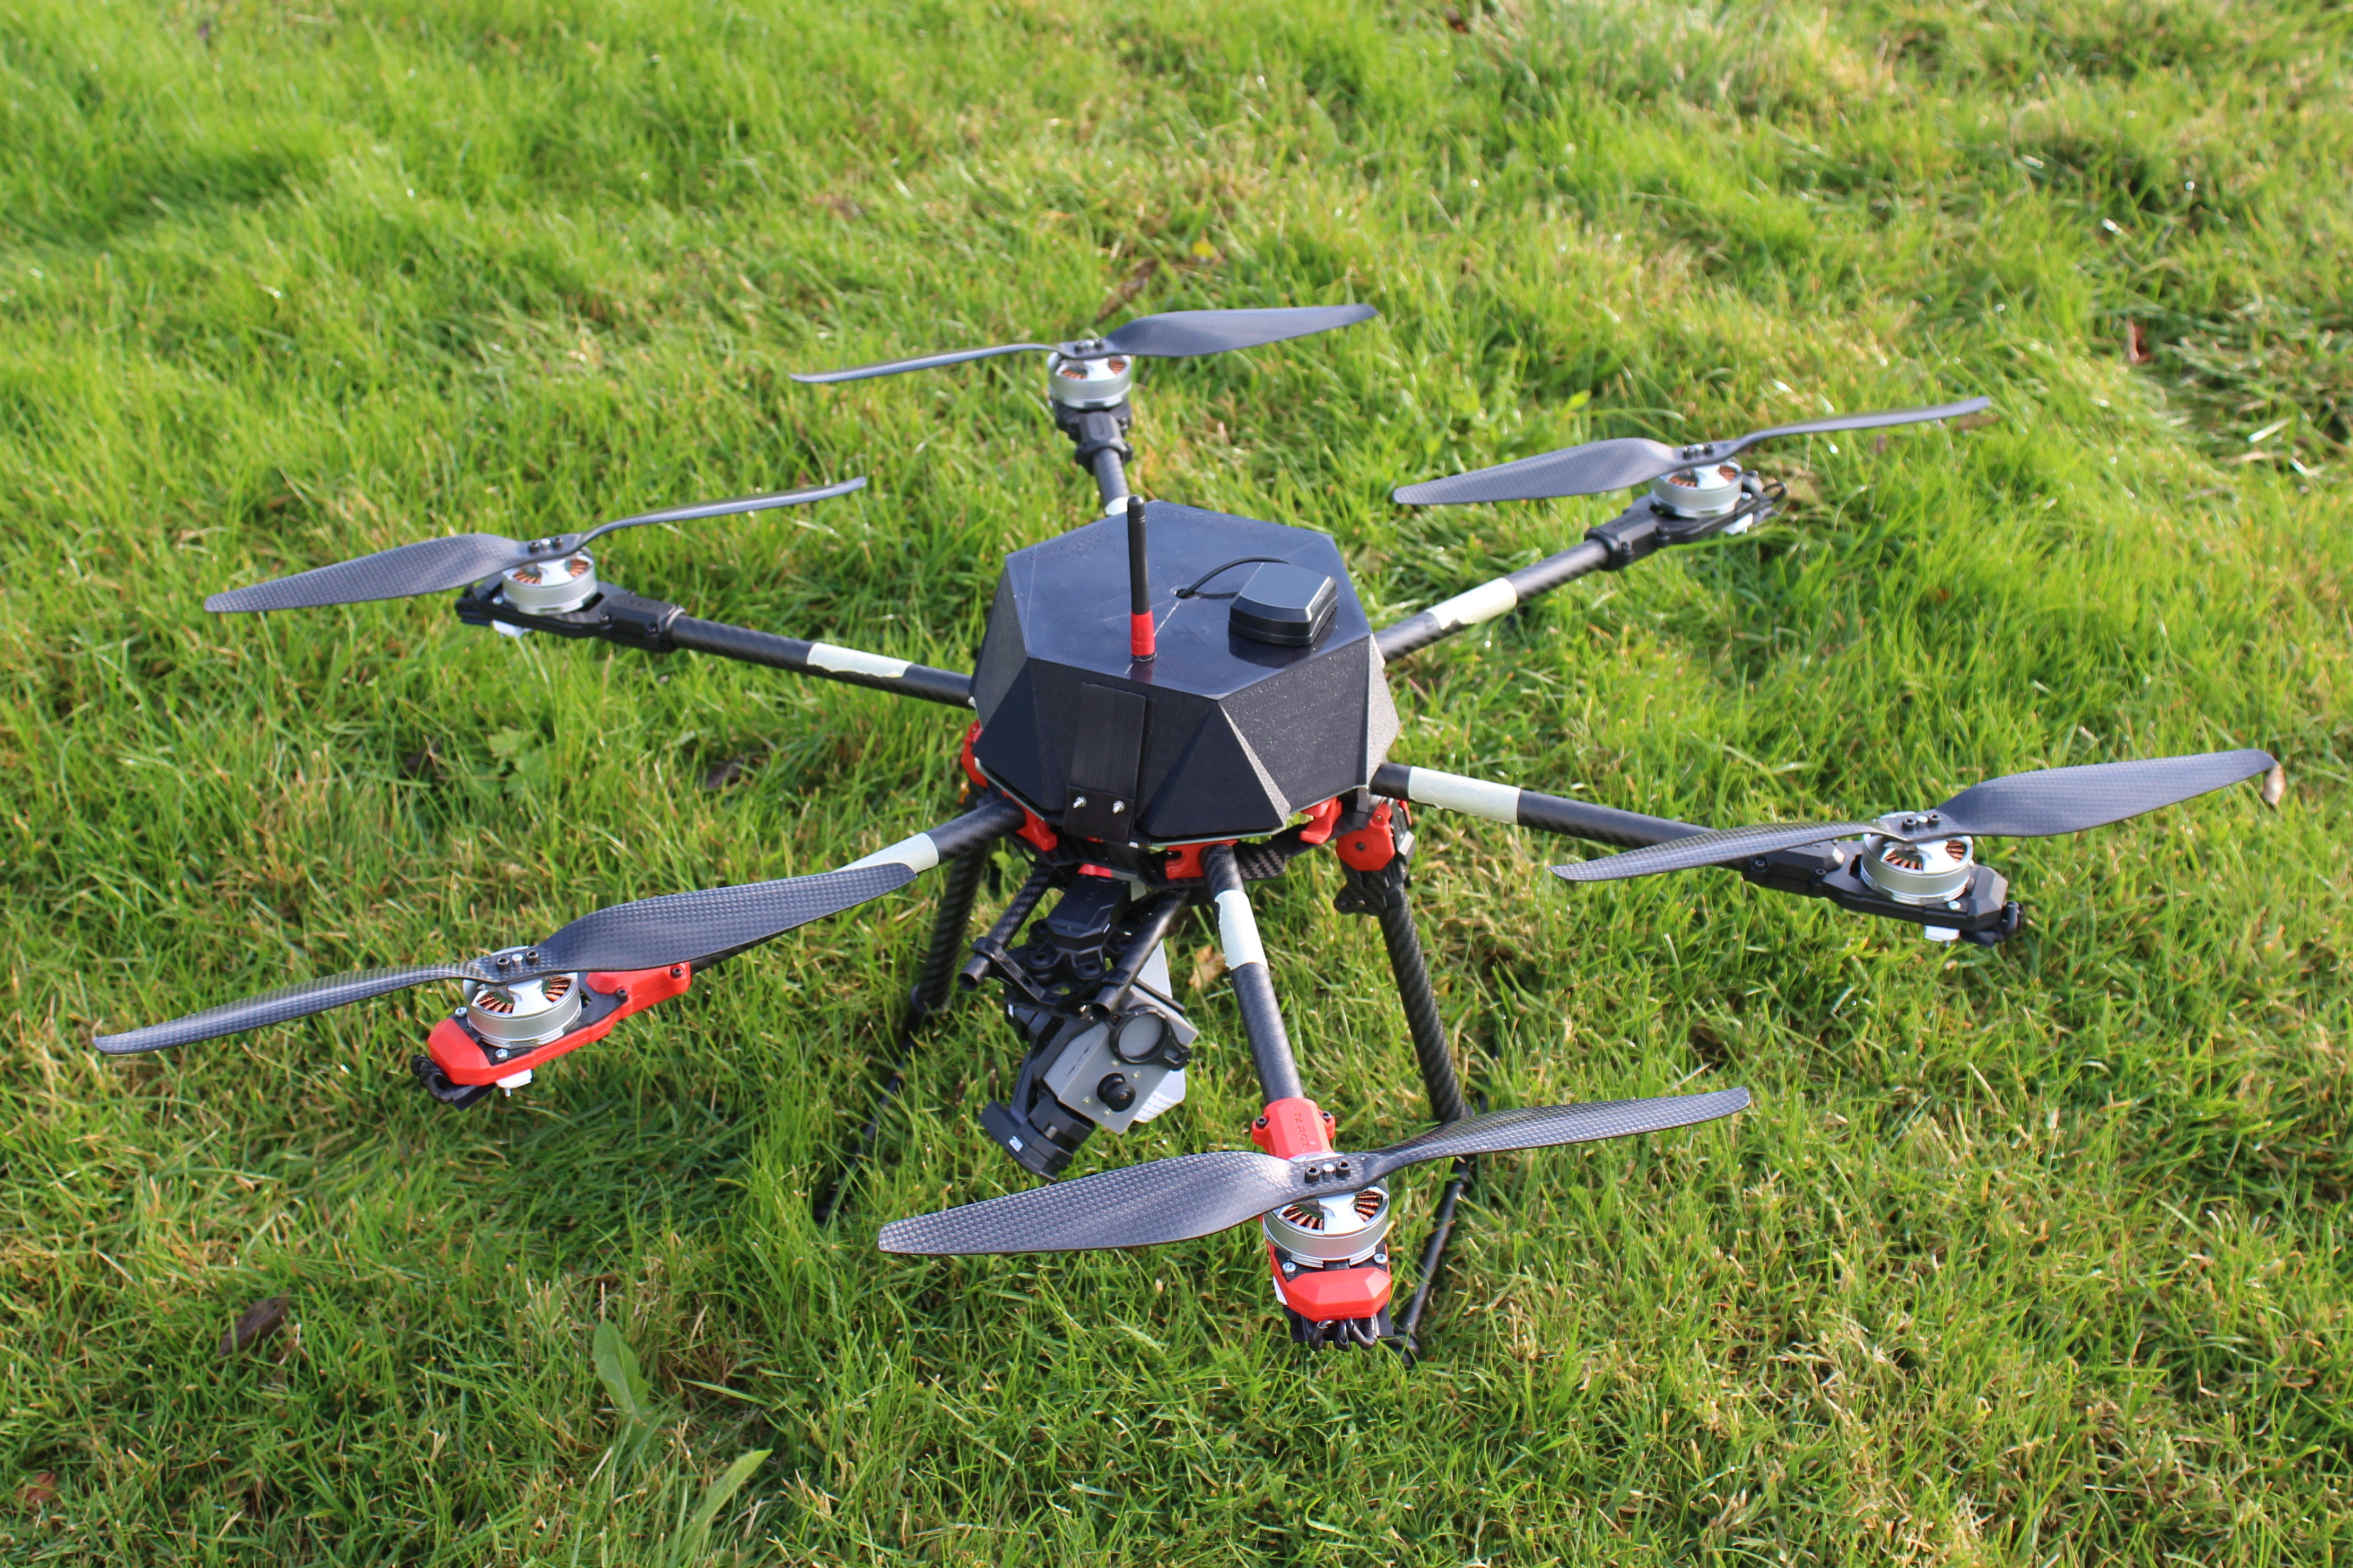
\includegraphics[width=0.45\linewidth]{images/jetson_drone.jpg}
    \end{figure}

    \begin{figure}
      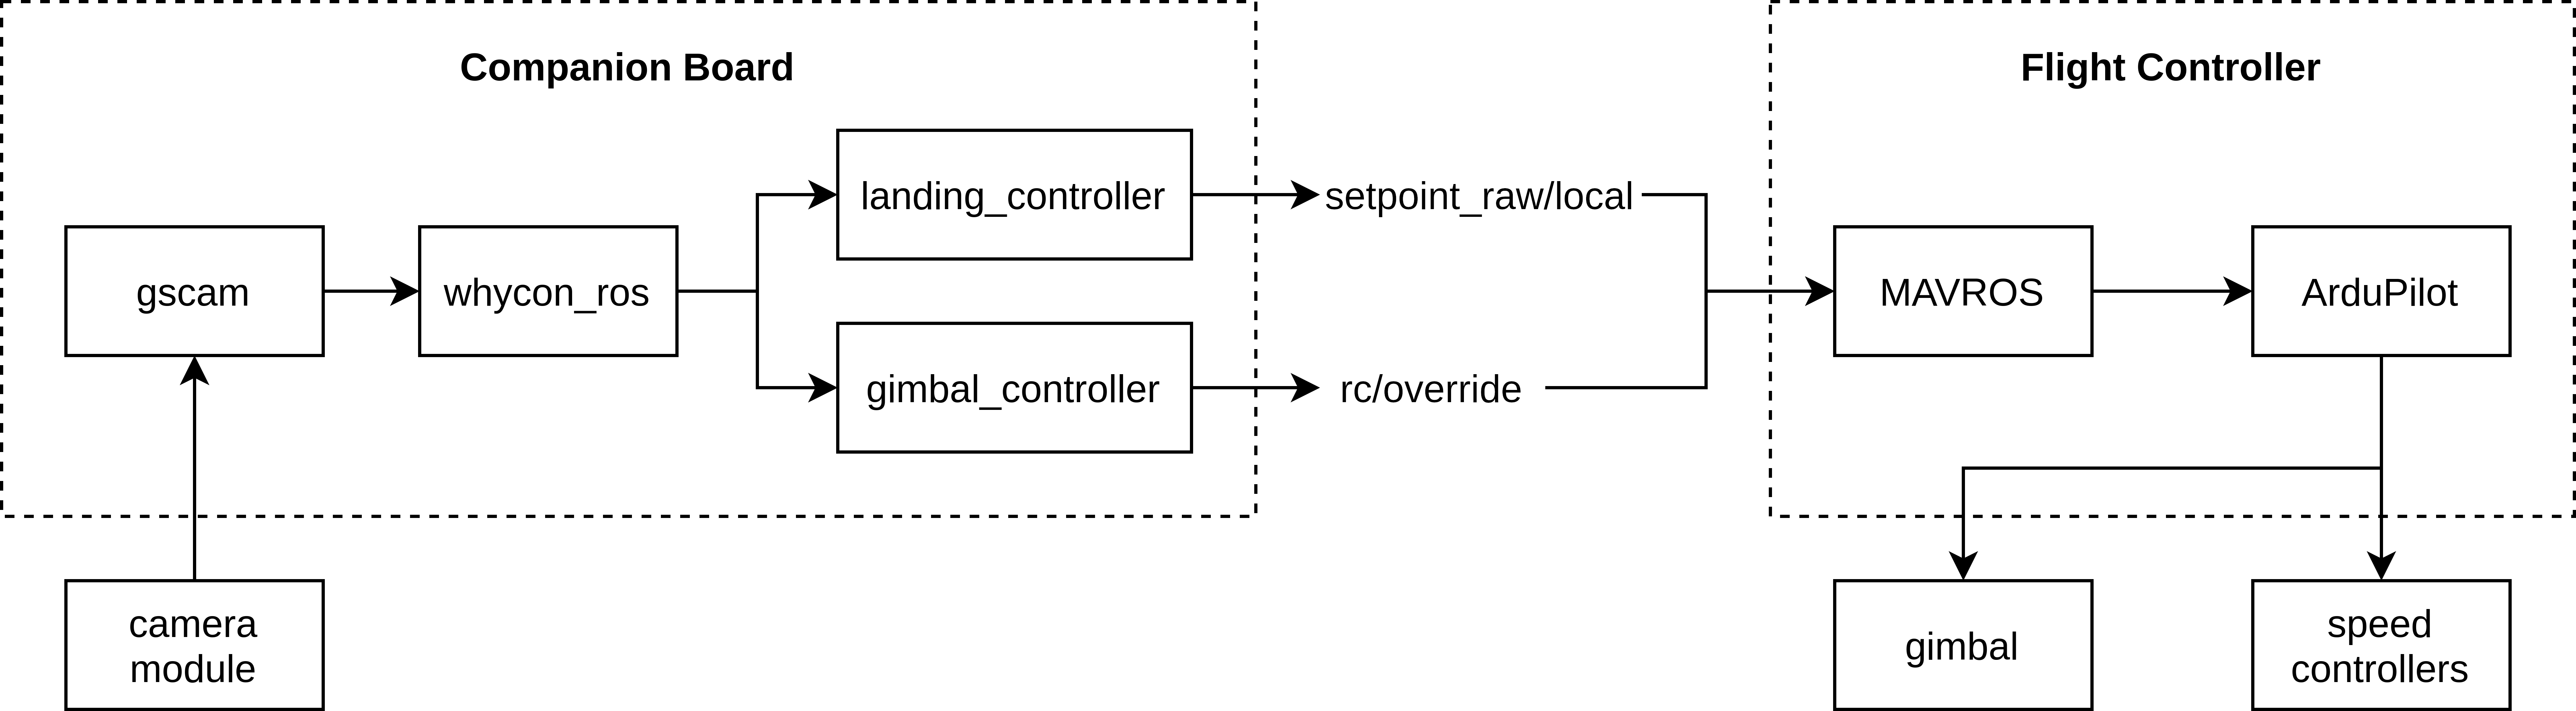
\includegraphics[width=\linewidth]{images/data_flow_opaque}
    \end{figure}

    The drones were able to track and approach the landing pads but did not execute successful landings because of low GPS accuracy
    (they often refused to enter autonomous mode) and issues with the marker systems (orientation ambiguity).
    This testing phase gave information on using drones autonomous in Iceland.

  \end{alertblock}

  \begin{block}{Orientation Ambiguity}
    Orientation ambiguity is the tendency of the orientation of fiducial markers to switch in a discontinuous way
    over time, as in the figure below, which represents the position of a landing pad relative to a drone.
    The east (left/right) and north (forward/backward) position targets have discontinuities as a result of orientation ambiguity.
    \vspace*{-0.5cm}
    \begin{figure}
      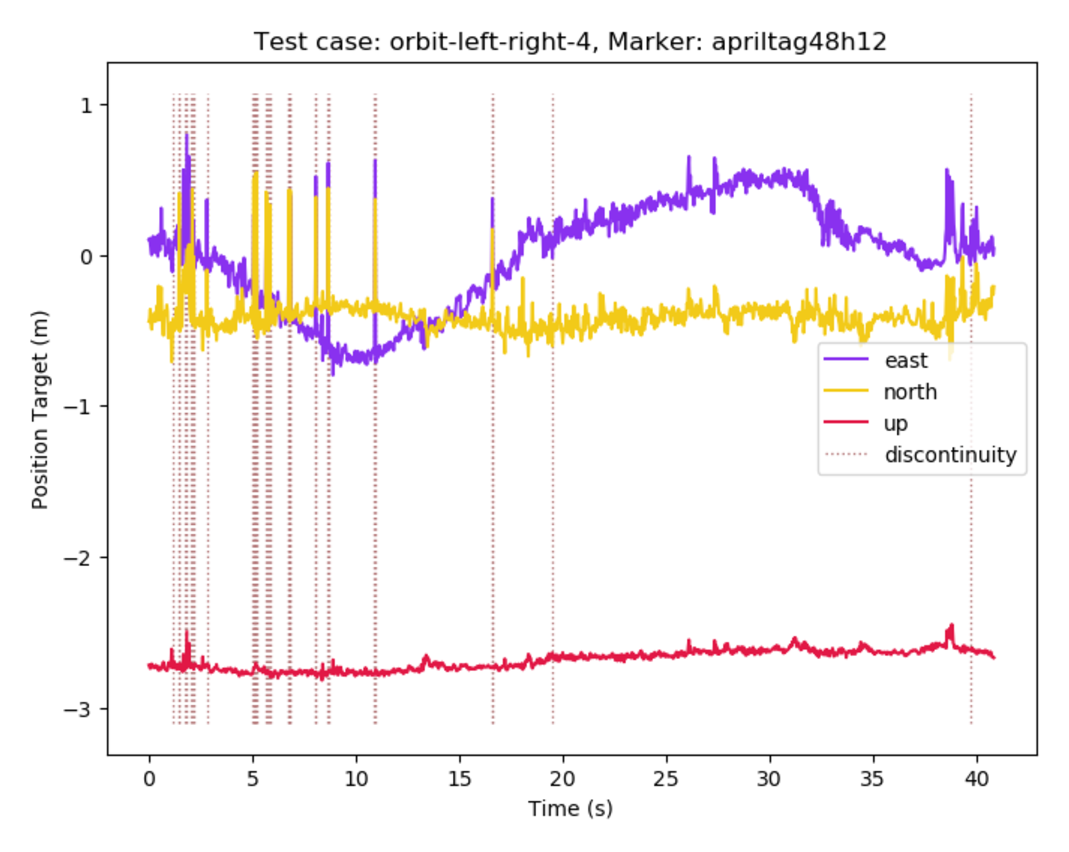
\includegraphics[width=0.65\linewidth]{images/orbit-left-right-4_apriltag48h12_position-target}
    \end{figure}

  \end{block}

  \end{column}

  \separatorcolumn

  \begin{column}{\colwidth}

  \begin{block}{Fiducial System Modifications}

    We use fiducial markers to detect our landing pads, and we have modified several fiducial systems that use the markers below for our purposes: to reduce the issue of
    orientation ambiguity, and to provide a fast detection rate (> 10 Hz) rate on embedded hardware.

    \begin{figure}[]
        \centering
        \begin{subfigure}[b]{0.22\linewidth}
            
\includegraphics[height=5cm]{./images/whycode_20_8}
            \caption{WhyCode}
            \label{figure:whycode_single}
        \end{subfigure}
        \begin{subfigure}[b]{0.25\linewidth}
            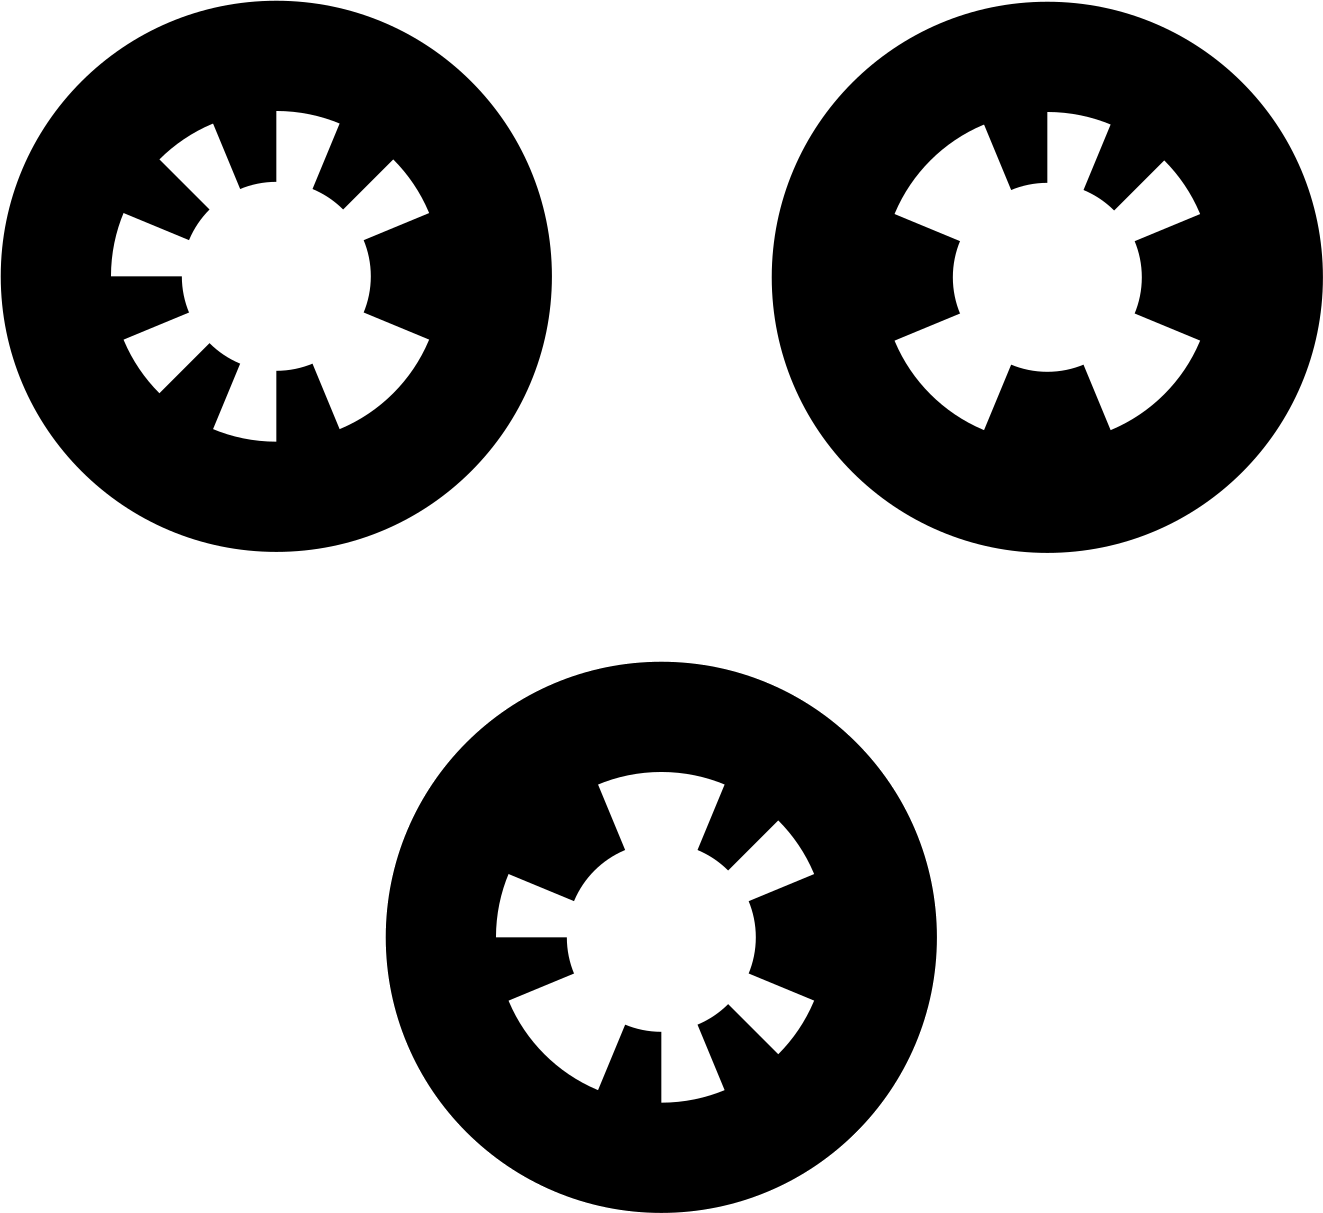
\includegraphics[height=5cm]{./images/whycode_multi}
            \caption{WhyCode Multi}
            \label{figure:whycode_bundle}
        \end{subfigure}
        \begin{subfigure}[b]{0.25\linewidth}
            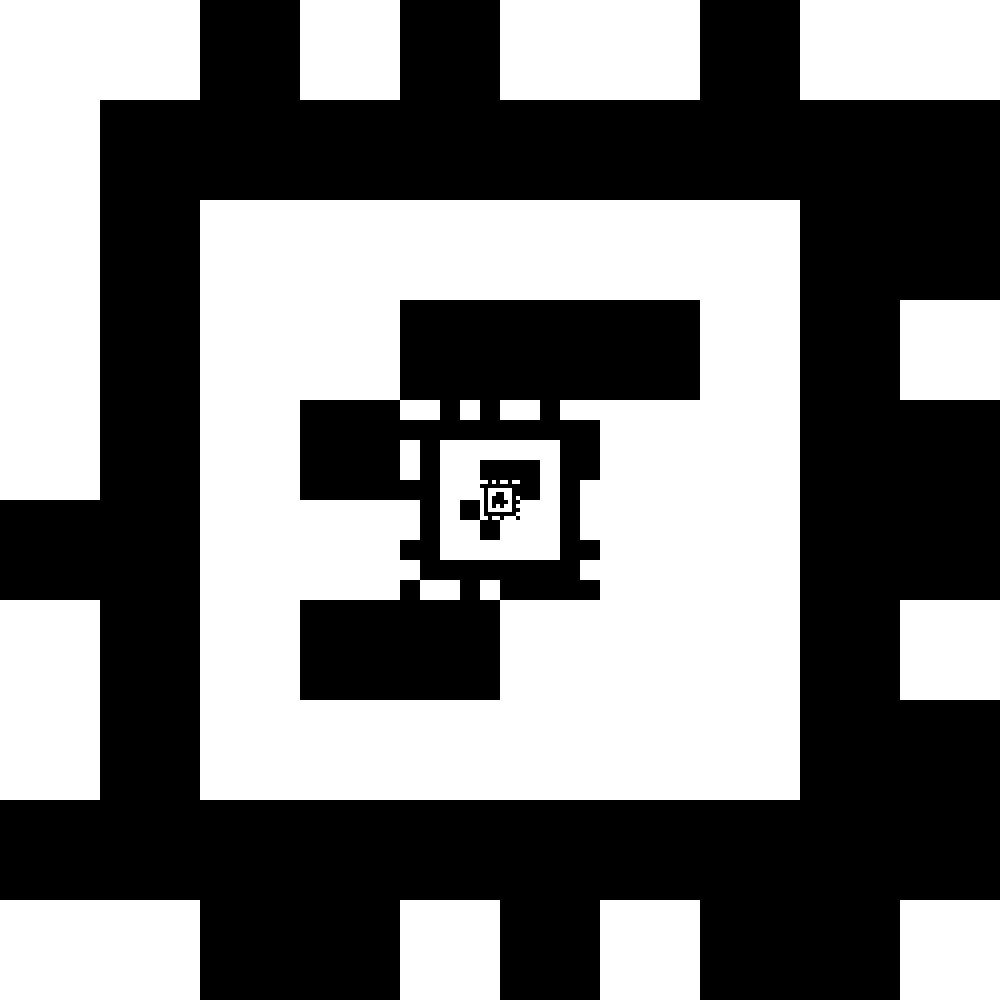
\includegraphics[height=5cm]{./images/tagCustom48h12_00002_00001_00000}
            \caption{AprilTag 48h12}
            \label{figure:apriltag48h12}
        \end{subfigure}
        \begin{subfigure}[b]{0.25\linewidth}
            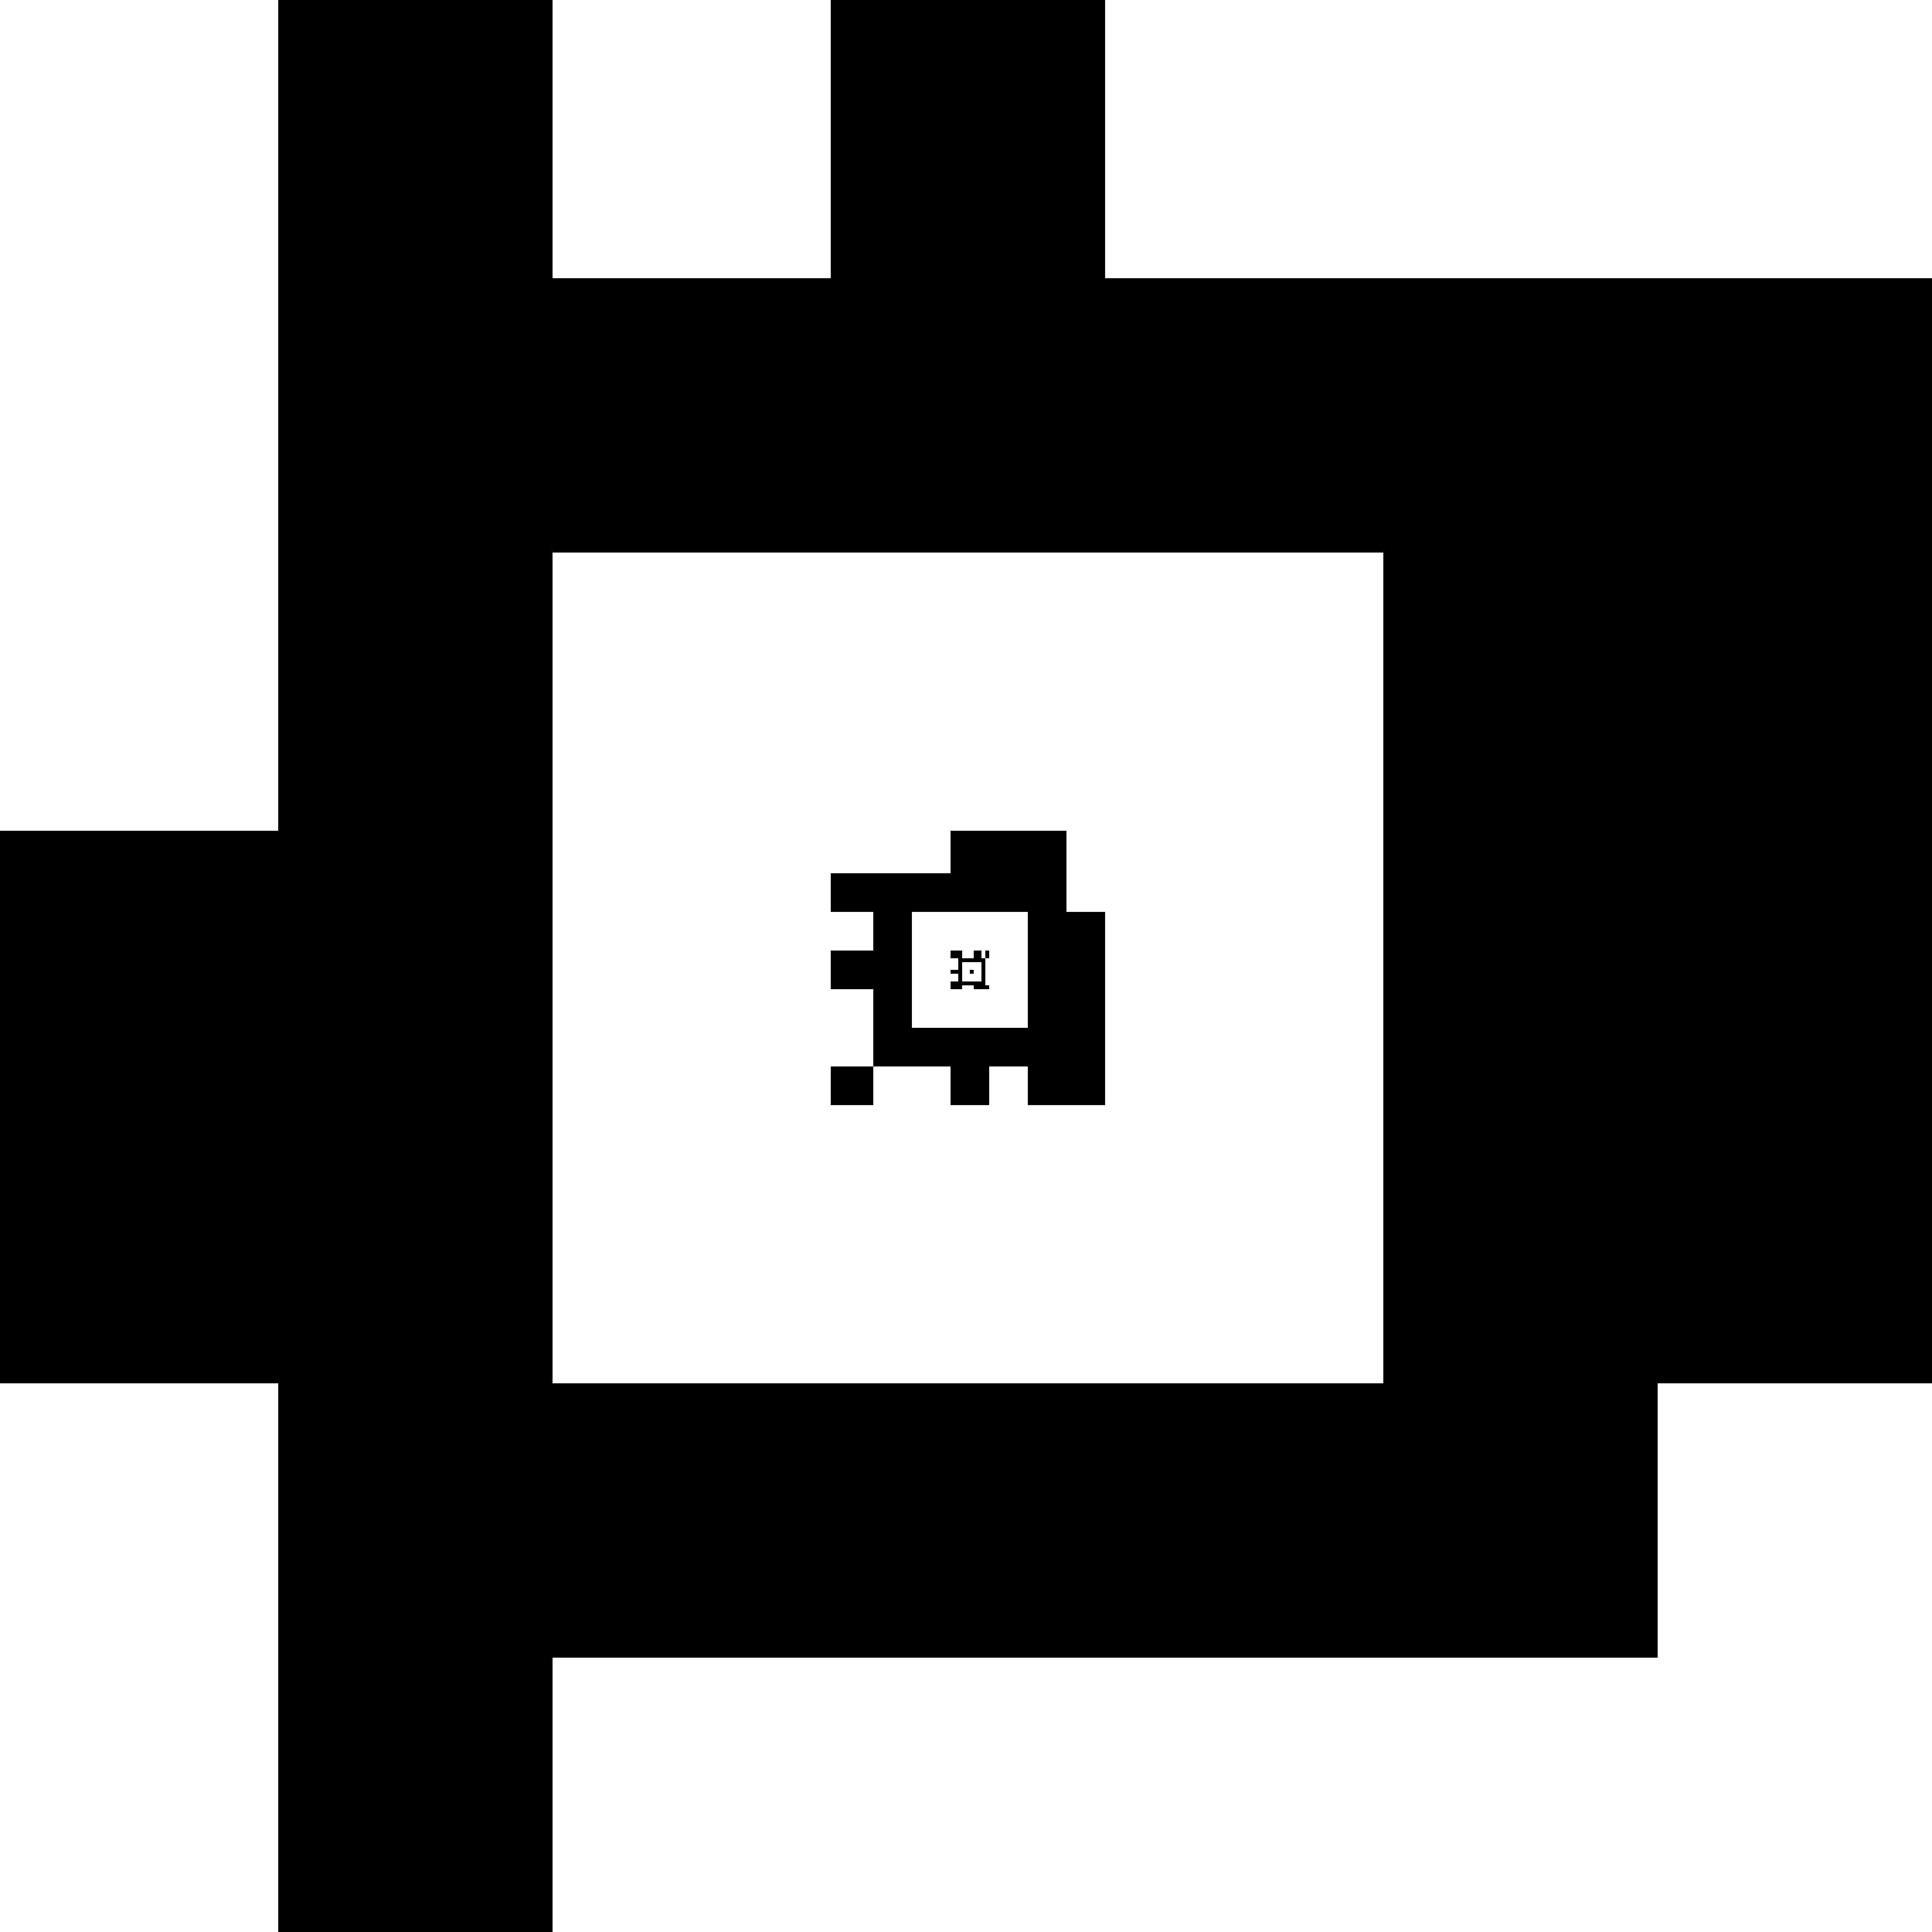
\includegraphics[height=5cm]{./images/tagCustom24h10_00002_00001_00000}
            \caption{AprilTag 24h10}
            \label{figure:apriltag24h10}
        \end{subfigure}
        \label{figure:marker_setup}
    \end{figure}
    \vspace*{-1.75cm}
    \textbf{WhyCode~Orig(inal)} samples the marker around the ID "teeth."
    \textbf{WhyCode~Ellipse} adds sampling locations allowing the system to better choose which circle is centered on the marker
    and reducing orientation ambiguity.

    \begin{figure}[]
        \centering
        \begin{subfigure}[b]{0.3\linewidth}
            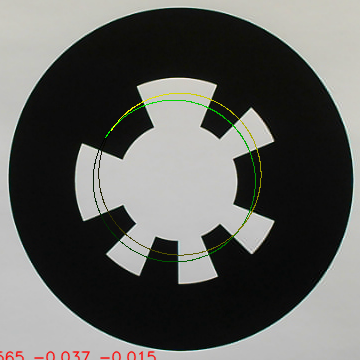
\includegraphics[width=\textwidth]{./images/whycode_orig_both_solutions_cropped}
            \caption{WhyCode Orig}
            \label{figure:whycode_orig}
        \end{subfigure}
        \begin{subfigure}[b]{0.3\linewidth}
            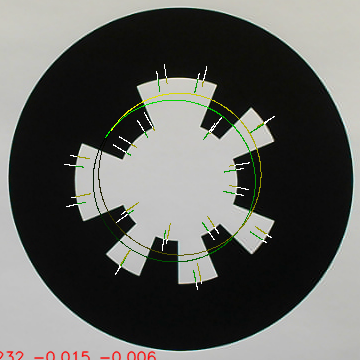
\includegraphics[width=\textwidth]{./images/whycode_ellipse_both_solutions_cropped}
            \caption{WhyCode Ellipse}
            \label{figure:whycode_ellipse}
        \end{subfigure}
    \end{figure}
    \vspace*{-1cm}
    \textbf{WhyCode~Multi} calculates the plane among 3+ markers, assumes they are coplanar, and uses the orientation
    from that plane, not those of the individual markers.
    \textbf{April~Tag~48h12} has a relatively low orientation ambiguity rate, but also has a low detection rate (about 2 Hz)
    on a Raspberry Pi 3, so we have made \textbf{April~Tag~24h10} with a smaller definition for quicker detection.
    The difference in detection rates is not shown below because this test was done on a Raspberry Pi 4 which can handle the system.
    \vspace*{-0.5cm}
    \begin{figure}[]
        \centering
        \begin{subfigure}[b]{0.49\linewidth}
            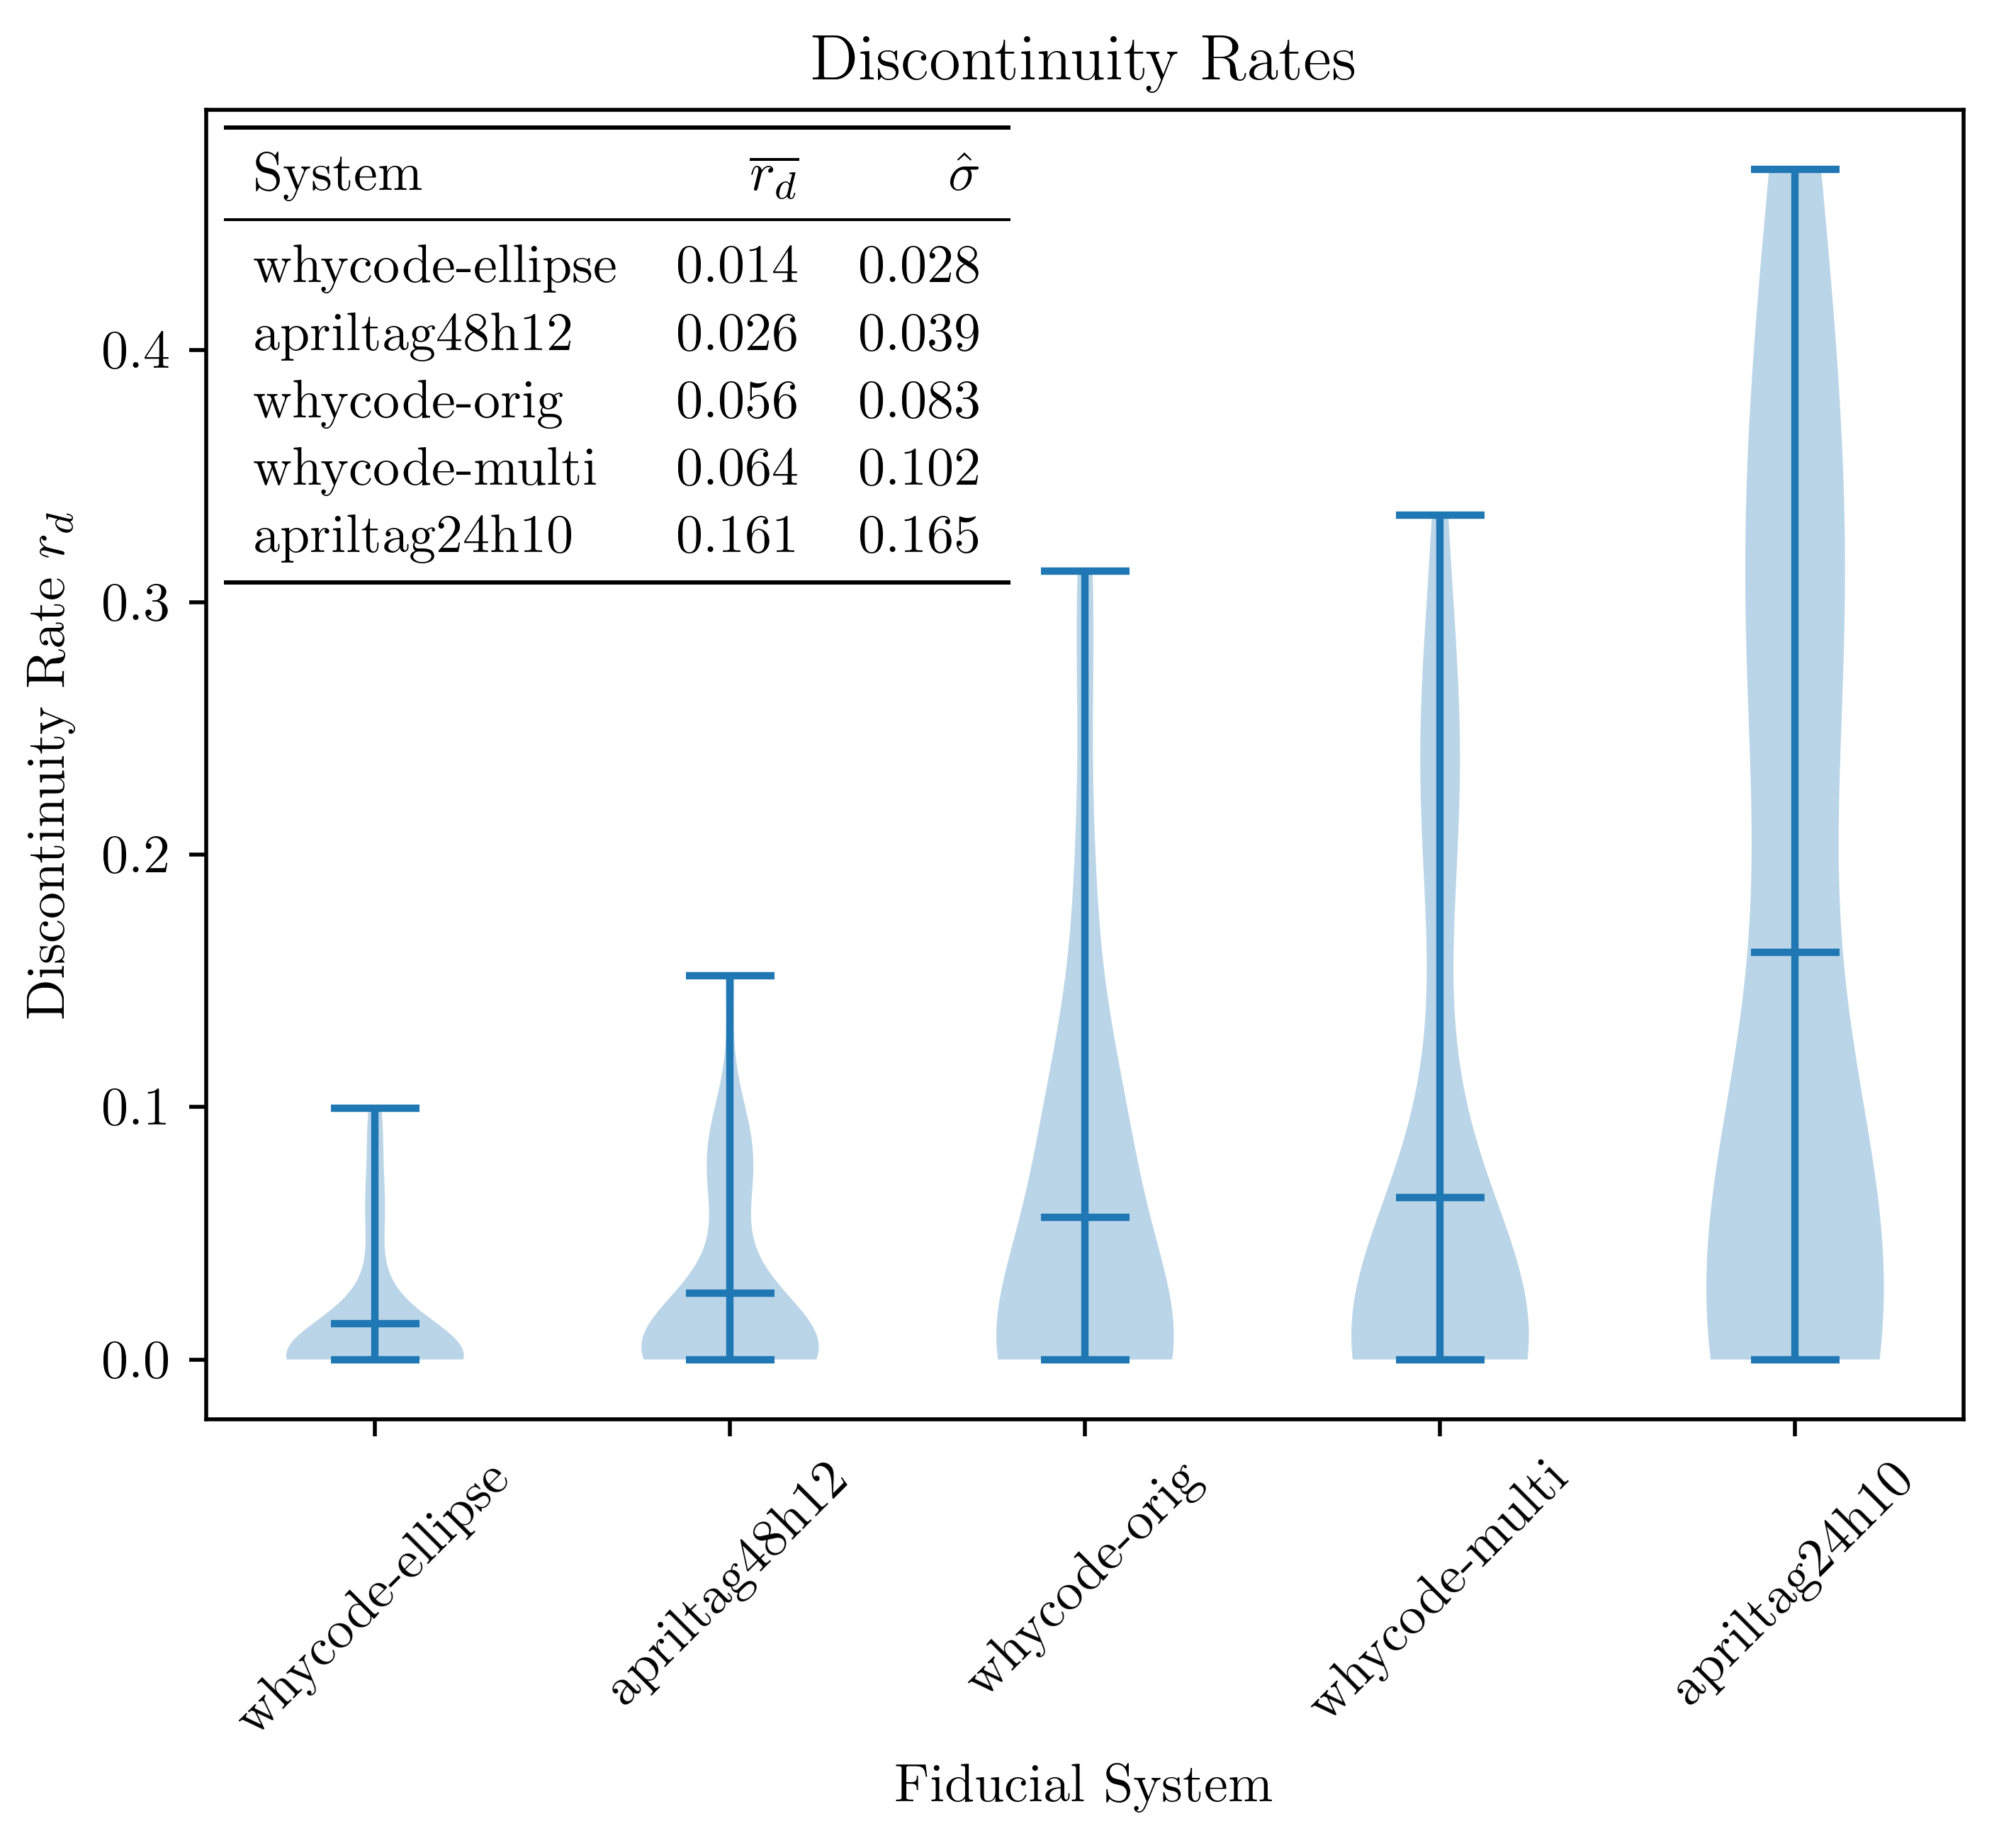
\includegraphics[width=\textwidth]{./images/violin_plot_five_member}
%            \caption{Distribution of discontinuity rates (lower is better). This denotes the number of discontinuities per detection.}
            \label{figure:violin_plot_five_member}
        \end{subfigure}
        \begin{subfigure}[b]{0.49\linewidth}
            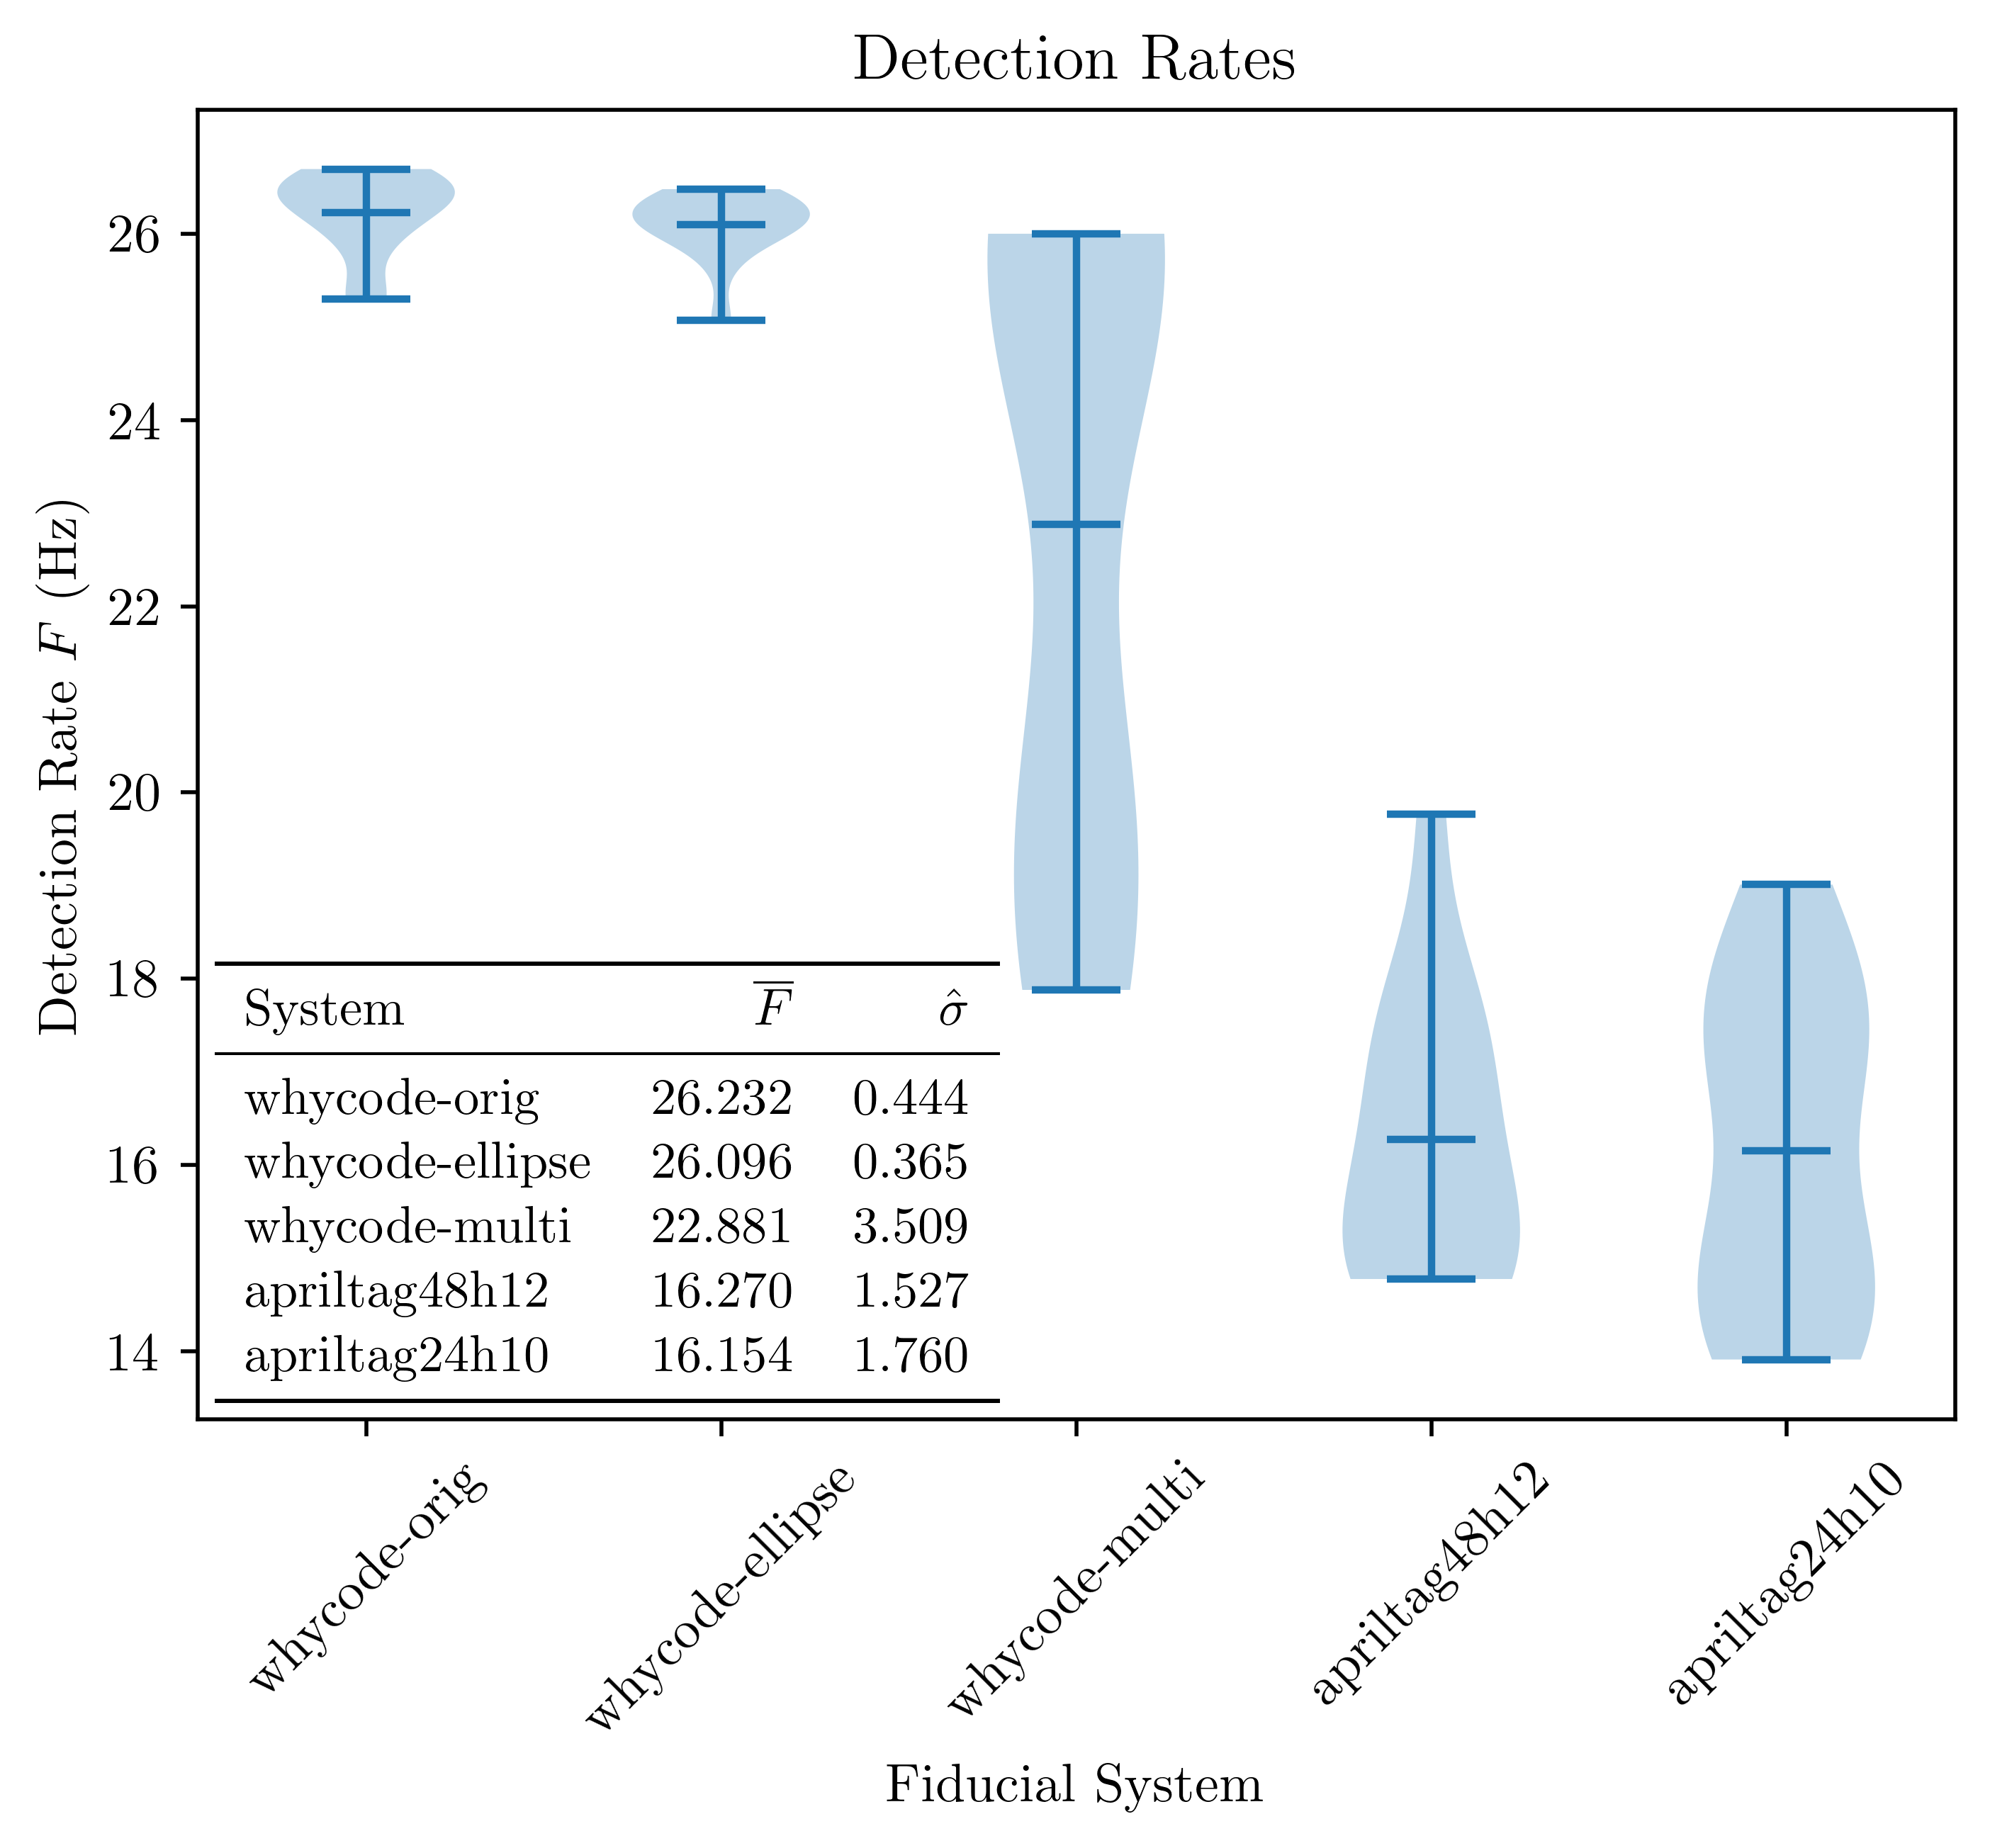
\includegraphics[width=\textwidth]{./images/violin_plot_speed_five_member}
%            \caption{Distribution of detection rates (higher is better). This denotes the number of detections per second.}
            \label{figure:violin_plot_speed_five_member}
        \end{subfigure}
    \end{figure}
    \vspace*{-1.5cm}
      We pick our modified WhyCode Ellipse and April Tag 48h12 as the best systems in terms of discontinuity rate,
      with each system having an acceptable detection rate.
      WhyCode Multi and April Tag 24h10 do not provide benefits in terms of discontinuity or detection rate.
  \end{block}

%  \begin{block}{A block containing an enumerated list}
%
%    Vivamus congue volutpat elit non semper. Praesent molestie nec erat ac
%    interdum. In quis suscipit erat. \textbf{Phasellus mauris felis, molestie
%    ac pharetra quis}, tempus nec ante. Donec finibus ante vel purus mollis
%    fermentum. Sed felis mi, pharetra eget nibh a, feugiat eleifend dolor. Nam
%    mollis condimentum purus quis sodales. Nullam eu felis eu nulla eleifend
%    bibendum nec eu lorem. Vivamus felis velit, volutpat ut facilisis ac,
%    commodo in metus.
%
%    \begin{enumerate}
%      \item \textbf{Morbi mauris purus}, egestas at vehicula et, convallis
%        accumsan orci. Orci varius natoque penatibus et magnis dis parturient
%        montes, nascetur ridiculus mus.
%      \item \textbf{Cras vehicula blandit urna ut maximus}. Aliquam blandit nec
%        massa ac sollicitudin. Curabitur cursus, metus nec imperdiet bibendum,
%        velit lectus faucibus dolor, quis gravida metus mauris gravida turpis.
%      \item \textbf{Vestibulum et massa diam}. Phasellus fermentum augue non
%        nulla accumsan, non rhoncus lectus condimentum.
%    \end{enumerate}
%
%  \end{block}

%  \begin{alertblock}{Fusce aliquam magna velit}
%
%    Et rutrum ex euismod vel. Pellentesque ultricies, velit in fermentum
%    vestibulum, lectus nisi pretium nibh, sit amet aliquam lectus augue vel
%    velit. Suspendisse rhoncus massa porttitor augue feugiat molestie. Sed
%    molestie ut orci nec malesuada. Sed ultricies feugiat est fringilla
%    posuere.
%
%    \begin{figure}
%      \centering
%      \begin{tikzpicture}
%        \begin{axis}[
%            scale only axis,
%            no markers,
%            domain=0:2*pi,
%            samples=100,
%            axis lines=center,
%            axis line style={-},
%            ticks=none]
%          \addplot[red] {sin(deg(x))};
%          \addplot[blue] {cos(deg(x))};
%        \end{axis}
%      \end{tikzpicture}
%      \caption{Another figure caption.}
%    \end{figure}
%
%  \end{alertblock}
%
%  \begin{block}{Nam cursus consequat egestas}
%
%    \begin{itemize}
%      \item \textbf{Sed consequat} id ante vel efficitur. Praesent congue massa
%        sed est scelerisque, elementum mollis augue iaculis.
%        \begin{itemize}
%          \item In sed est finibus, vulputate
%            nunc gravida, pulvinar lorem. In maximus nunc dolor, sed auctor eros
%            porttitor quis.
%          \item Fusce ornare dignissim nisi. Nam sit amet risus vel lacus
%            tempor tincidunt eu a arcu.
%          \item Donec rhoncus vestibulum erat, quis aliquam leo
%            gravida egestas.
%        \end{itemize}
%      \item \textbf{Sed luctus, elit sit amet} dictum maximus, diam dolor
%        faucibus purus, sed lobortis justo erat id turpis.
%      \item \textbf{Pellentesque facilisis dolor in leo} bibendum congue.
%        Maecenas congue finibus justo, vitae eleifend urna facilisis at.
%    \end{itemize}
%
%  \end{block}

\end{column}

\separatorcolumn

\begin{column}{\colwidth}

  \begin{alertblock}{Autonomous Landing with DJI Spark}

    We have retested the autonomous landing techniques will all previous fiducial systems, using a small DJI Spark
      so that the tests can be conducted indoors.
      This required the development of an Android App to interface with the DJI Mobile SDK for autonomous control, shown below.
      All systems but WhyCode Multi allowed successful autonomous landings.
      Scan the QR code for autonomous landing demonstrations.
      \begin{figure}
          \centering
          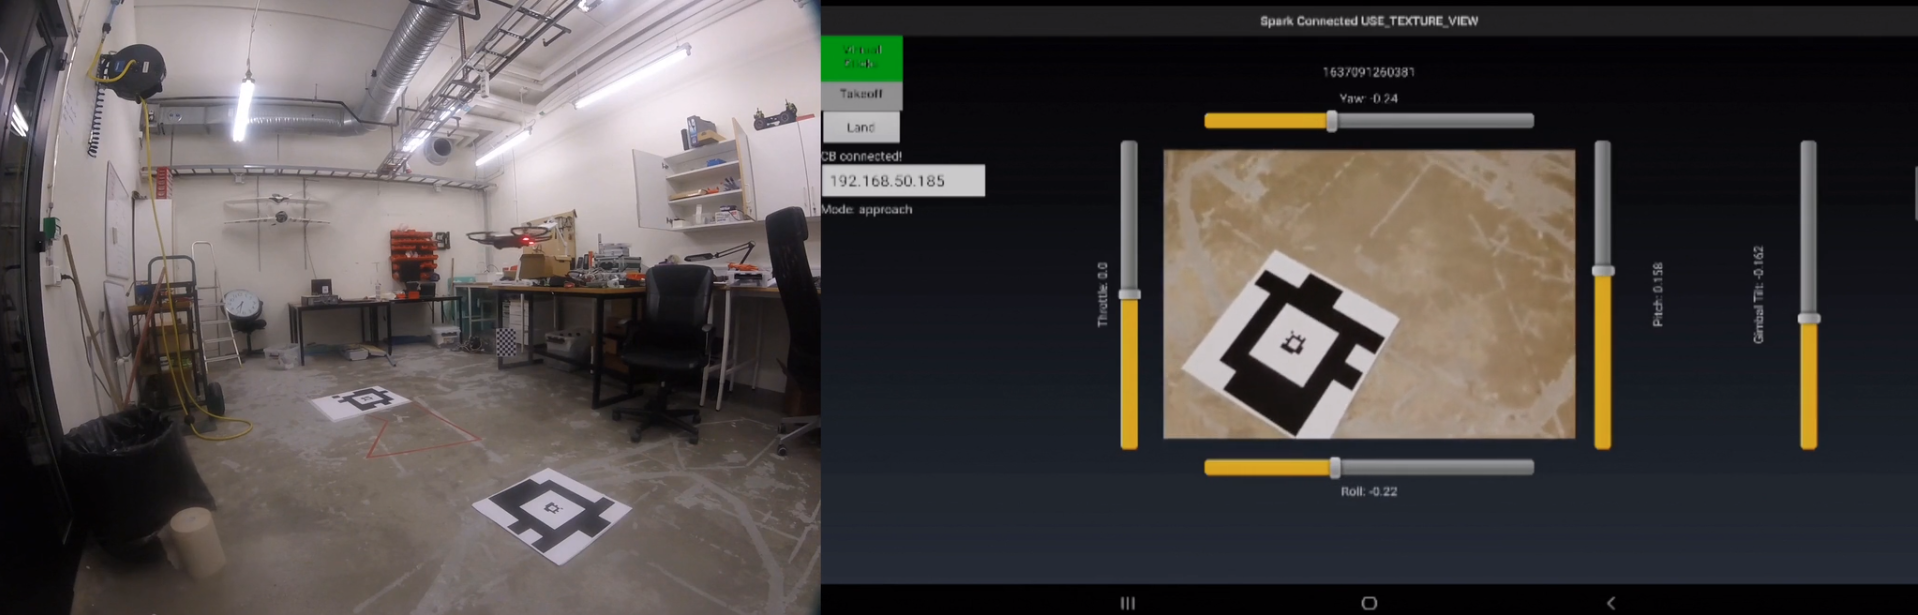
\includegraphics[width=\linewidth]{images/demo_screenshot}
      \end{figure}

  \end{alertblock}

  \begin{block}{Future Work}

      Overall, the work moving forward will focus on generating a new autonomous landing method that uses terrain analysis,
      so that the landing will not be limited to known landing sites.
      However, it will use a unified set of sensors so that the drone will be able to use the existing fiducial systems
      whenever landing at a known landing site.
      The method will also use the same paradigm of aiming a sensor via a gimbal, detecting a landing site,
      and directing the drone using velocity or position commands.
      We will first conduct landing experiments in simulation, then slowly move them onto physical drones.
      \textbf{The scope of the project will be limited by the available sensors and testing environments.}
      The sensors include RealSense depth cameras and LIDAR modules, which also provide RGB cameras for integration with our existing landing algorithm.
      Additionally, they have IMUs for reliable orientation estimation, which will help eliminate the orientation ambiguity problem.
      We will do the following tasks:
      \vspace*{-0.5cm}
    \begin{itemize}
        \item \textbf{Drone Upgrades:} add optical flow and LIDAR sensors to hexacopters for GPS-free autonomous flight.
        \item \textbf{Re-test autonomous landing:} use the hexacopters, test outdoors.
        \item \textbf{Develop free-form landing algorithm:} in simulation, use depth/LIDAR sensors to analyze terrain and find safe landing spots in unknown locations.
        \item \textbf{Add depth camera to drones:} build a gimbal adapter, supplement power system and integrate with onboard hardware.
        \item \textbf{Test in the real world:} we limit the scope of the tests to rural Icelandic environments where it is most applicable to our work.
    \end{itemize}
    \vspace*{-0.5cm}
    \textbf{Publications:} We have submitted one paper on the fiducial system modifications, and another in progress describing the results of the proof of concept with the DJI Spark.
      Anticipated publications include one paper detailing the free-form landing method, and one detailing real world tests of the unified system with both fiducial and free-form landing.

  \end{block}



  \begin{block}{References}

    \nocite{*}
    \footnotesize{\bibliographystyle{plain}\bibliography{poster}}

  \end{block}

\end{column}

\separatorcolumn
\end{columns}
\end{frame}

\end{document}
